\documentclass{standalone}
\usepackage{tikz}

\begin{document}

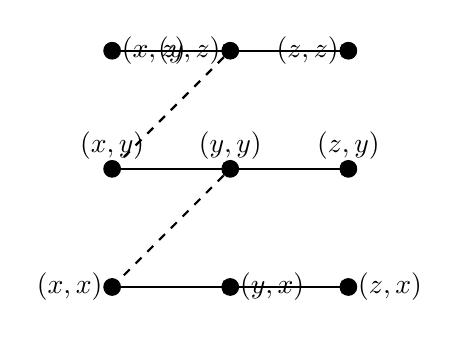
\begin{tikzpicture}[scale=1.5]
    % Define coordinates
    \coordinate (A) at (0,0);
    \coordinate (B) at (1,0);
    \coordinate (C) at (2,0);
    \coordinate (D) at (0,1);
    \coordinate (E) at (1,1);
    \coordinate (F) at (2,1);
    \coordinate (G) at (0,2);
    \coordinate (H) at (1,2);
    \coordinate (I) at (2,2);

    % Draw nodes with labels
    \filldraw[black] (A) circle (2pt) node[anchor=east] {$(x,x)$};
    \filldraw[black] (B) circle (2pt) node[anchor=west] {$(y,x)$};
    \filldraw[black] (C) circle (2pt) node[anchor=west] {$(z,x)$};
    \filldraw[black] (D) circle (2pt) node[anchor=south] {$(x,y)$};
    \filldraw[black] (E) circle (2pt) node[anchor=south] {$(y,y)$};
    \filldraw[black] (F) circle (2pt) node[anchor=south] {$(z,y)$};
    \filldraw[black] (G) circle (2pt) node[anchor=west] {$(x,z)$};
    \filldraw[black] (H) circle (2pt) node[anchor=east] {$(y,z)$};
    \filldraw[black] (I) circle (2pt) node[anchor=east] {$(z,z)$};

    % Draw arrows
    \draw[->, thick] (A) -- (B);
    \draw[->, thick] (B) -- (C);
    \draw[->, thick] (D) -- (E);
    \draw[->, thick] (E) -- (F);
    \draw[->, thick] (G) -- (H);
    \draw[->, thick] (H) -- (I);
    \draw[dashed, thick] (A) -- (E);
    \draw[dashed, thick] (D) -- (H);
    \draw[dashed, thick] (G) -- (I);
\end{tikzpicture}

\end{document}